\subsubsection{Casos de uso del sistema}

Los casos de uso del sistema representan las interacciones entre los actores y las funcionalidades clave de la aplicación. A través de estos, se detallan los escenarios en los que los usuarios, administradores y otros actores relevantes interactúan con el sistema para cumplir con los objetivos propuestos. A continuación en la \autoref{fig:system-use-cases-diagram}, se presenta un diagrama de caso de uso que proporciona una vista general de las acciones que los usuarios pueden realizar, contribuyendo a una mejor comprensión de los requisitos funcionales definidos.

\begin{figure}[H]
    \centering
    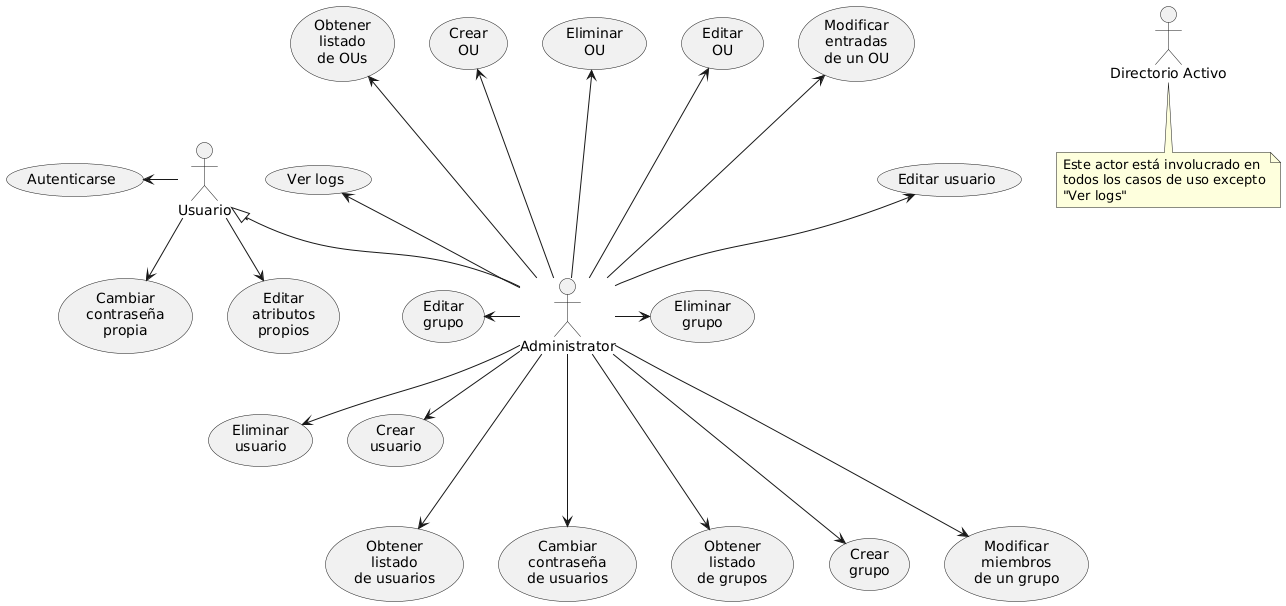
\includegraphics[width=\linewidth]{images/puml/system-diagram/system-diagram.png}
    \caption{Diagrama de casos de uso del sistema}
    \label{fig:system-use-cases-diagram}
\end{figure}